\usetikzlibrary{shapes.geometric}
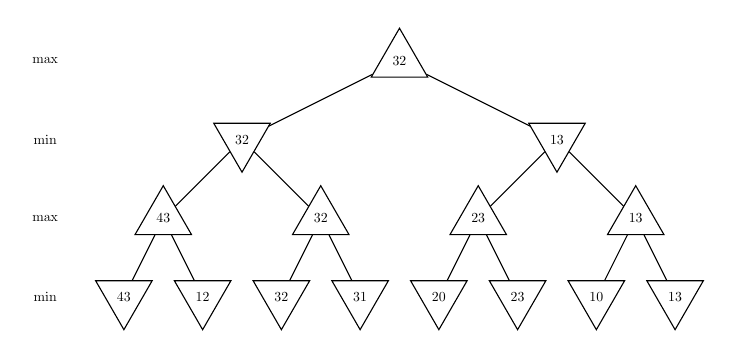
\begin{tikzpicture}[every node/.style={scale=0.5}]
\tikzstyle{treenode}=[draw,regular polygon, regular polygon sides=3,shape border uses incircle];
\tikzstyle{maxnode}=[treenode];
\tikzstyle{minnode}=[treenode,shape border rotate=60];
\node [maxnode] (v1) at (-0.5,2) {32};
\node [minnode] (v2) at (-2.5,1) {32};
\node [minnode] (v9) at (1.5,1) {13};
\node [maxnode] (v3) at (-3.5,0) {43};
\node [maxnode] (v4) at (-1.5,0) {32};
\node [maxnode] (v10) at (0.5,0) {23};
\node [maxnode] (v11) at (2.5,0) {13};
\node [minnode] (v5) at (-4,-1) {43};
\node [minnode] (v6) at (-3,-1) {12};
\node [minnode] (v7) at (-2,-1) {32};
\node [minnode] (v8) at (-1,-1) {31};
\node [minnode] (v12) at (0,-1) {20};
\node [minnode] (v13) at (1,-1) {23};
\node [minnode] (v14) at (2,-1) {10};
\node [minnode] (v15) at (3,-1) {13};
\draw  (v1) edge (v2);
\draw  (v2) edge (v3);
\draw  (v2) edge (v4);
\draw  (v3) edge (v5);
\draw  (v3) edge (v6);
\draw  (v4) edge (v7);
\draw  (v4) edge (v8);
\draw  (v1) edge (v9);
\draw  (v9) edge (v10);
\draw  (v9) edge (v11);
\draw  (v10) edge (v12);
\draw  (v10) edge (v13);
\draw  (v11) edge (v14);
\draw  (v11) edge (v15);
\node  at (-5,2) {max};
\node at (-5,1) {min};
\node at (-5,0) {max};
\node at (-5,-1) {min};
\end{tikzpicture}